\chapter{La vie au fil des saisons}\label{ch:g6:life-through-seasons}

Photographie le même marronnier le premier de chaque mois et
épingle les douze images à la suite~: \omterm{def:g1:plants-around-us:tree}{branches} nues, \omterm{def:g6:life-through-seasons:buds}{bourgeons},
\omterm{def:g1:plants-around-us:parts}{feuilles}, chandelles de \omterm{def:g3:flowers-fruits-seeds:parts}{fleurs}, marrons, or, \omterm{def:g1:plants-around-us:tree}{branches} nues de
nouveau. Rien n'a bougé --- l'arbre est resté immobile toute
l'année --- et pourtant tout a changé.
\Cref{ch:g3:animals-through-seasons} suivait les \omterm{def:g1:animals-around-us:animal}{animaux} au fil de
l'année~; maintenant, avec des \omterm{def:g1:the-five-senses:sense}{yeux} de releveur, nous suivons
l'\omterm{def:g6:exploring-our-environment:components}{environnement} entier, en commençant par les \omterm{def:g1:plants-around-us:plant}{plantes}.

\section{L'environnement change avec les saisons}

\begin{proposition}[Le changement saisonnier des conditions]\label{prop:g6:life-through-seasons:conditions}
Au fil de l'année, les \omterm{def:g6:exploring-our-environment:conditions}{conditions} d'un \omterm{def:g6:exploring-our-environment:components}{environnement}
(\cref{def:g6:exploring-our-environment:conditions}) varient
largement~: les jours raccourcissent et rallongent, les \omterm{def:g6:exploring-our-environment:conditions}{températures}
baissent et remontent, l'\omterm{def:g6:exploring-our-environment:conditions}{humidité} du sol suit la pluie et la
sécheresse. Un site relevé en janvier et en juin donne deux lignes
différentes dans le tableau --- donc, d'après
\cref{prop:g6:exploring-our-environment:decide}, attends-toi à deux
distributions d'habitants différentes.
\end{proposition}
\admitted

\begin{example}[Une haie, deux relevés]\label{ex:g6:life-through-seasons:hedge}
La haie du chemin, relevée deux fois. Juin~: feuillage dense, dix
\omterm{def:g5:biodiversity:species}{espèces} de \omterm{def:g1:plants-around-us:plant}{plantes} en \omterm{def:g3:flowers-fruits-seeds:parts}{fleur} à son pied, abeilles bruyantes, merles
qui nichent, escargots après la pluie. Janvier~: rameaux nus, du
vert réduit au lierre et à la mousse, aucun insecte en vol, merles
qui fouillent la litière de \omterm{def:g1:plants-around-us:parts}{feuilles}, escargots scellés dans leur
\omterm{def:g1:animals-around-us:covering}{coquille} au fond du talus. Même endroit, même liste de composantes
--- vivants, minéral, traces --- mais la colonne des vivants s'est
transformée.
\end{example}

\section{Comment les plantes passent la mauvaise saison}

\begin{definition}[Caducs et persistants]\label{def:g6:life-through-seasons:trees}
Les arbres se partagent selon leur réponse à l'hiver~:
\begin{itemize}
  \item les arbres à \omterm{def:g1:plants-around-us:parts}{feuilles} \emph{caduques}\index{caduc} ---
        chêne, marronnier, hêtre --- perdent toutes leurs \omterm{def:g1:plants-around-us:parts}{feuilles}
        en automne et restent nus~;
  \item les arbres à \omterm{def:g1:plants-around-us:parts}{feuilles} \emph{persistantes}\index{persistant}
        --- pin, houx, lierre sur le mur --- gardent tout l'hiver
        des \omterm{def:g1:plants-around-us:parts}{feuilles} qui travaillent, en général coriaces, cireuses
        ou en forme d'aiguilles
        (\cref{prop:g3:sorting-living-things:plants} avait déjà
        rencontré les aiguilles).
\end{itemize}
\end{definition}

\begin{definition}[Bourgeons]\label{def:g6:life-through-seasons:buds}
Un arbre à \omterm{def:g1:plants-around-us:parts}{feuilles} \omterm{def:g6:life-through-seasons:trees}{caduques} n'est pas mort en hiver~: le printemps
suivant est déjà rangé sur ses rameaux sous forme de
\emph{bourgeons}\index{bourgeon} --- de minuscules pousses
complètes, \omterm{def:g1:plants-around-us:parts}{feuilles} pliées menu, enveloppées d'\omterm{def:g1:animals-around-us:covering}{écailles} à l'épreuve
du temps. Les \omterm{def:g1:plants-around-us:parts}{feuilles} «~nouvelles~» du printemps ont été bâties
l'été d'avant~; le bourgeon est leur rangement d'hiver.
\end{definition}

\begin{example}[Ouvrir un bourgeon de marronnier]\label{ex:g6:life-through-seasons:bud}
Les gros \omterm{def:g6:life-through-seasons:buds}{bourgeons} collants du marronnier s'ouvrent bien sous une
lame (l'affaire d'un adulte)~: sous les \omterm{def:g1:animals-around-us:covering}{écailles} vernies, tassées
dans un duvet cotonneux, reposent des \omterm{def:g1:plants-around-us:parts}{feuilles} miniatures pliées ---
parfaites, pâles, en attente. Un rameau coupé en février et mis dans
l'eau à l'intérieur «~débourre~» des semaines en avance~: les pousses
étaient finies~; il ne manquait que la chaleur.
\end{example}

\begin{omfigure}
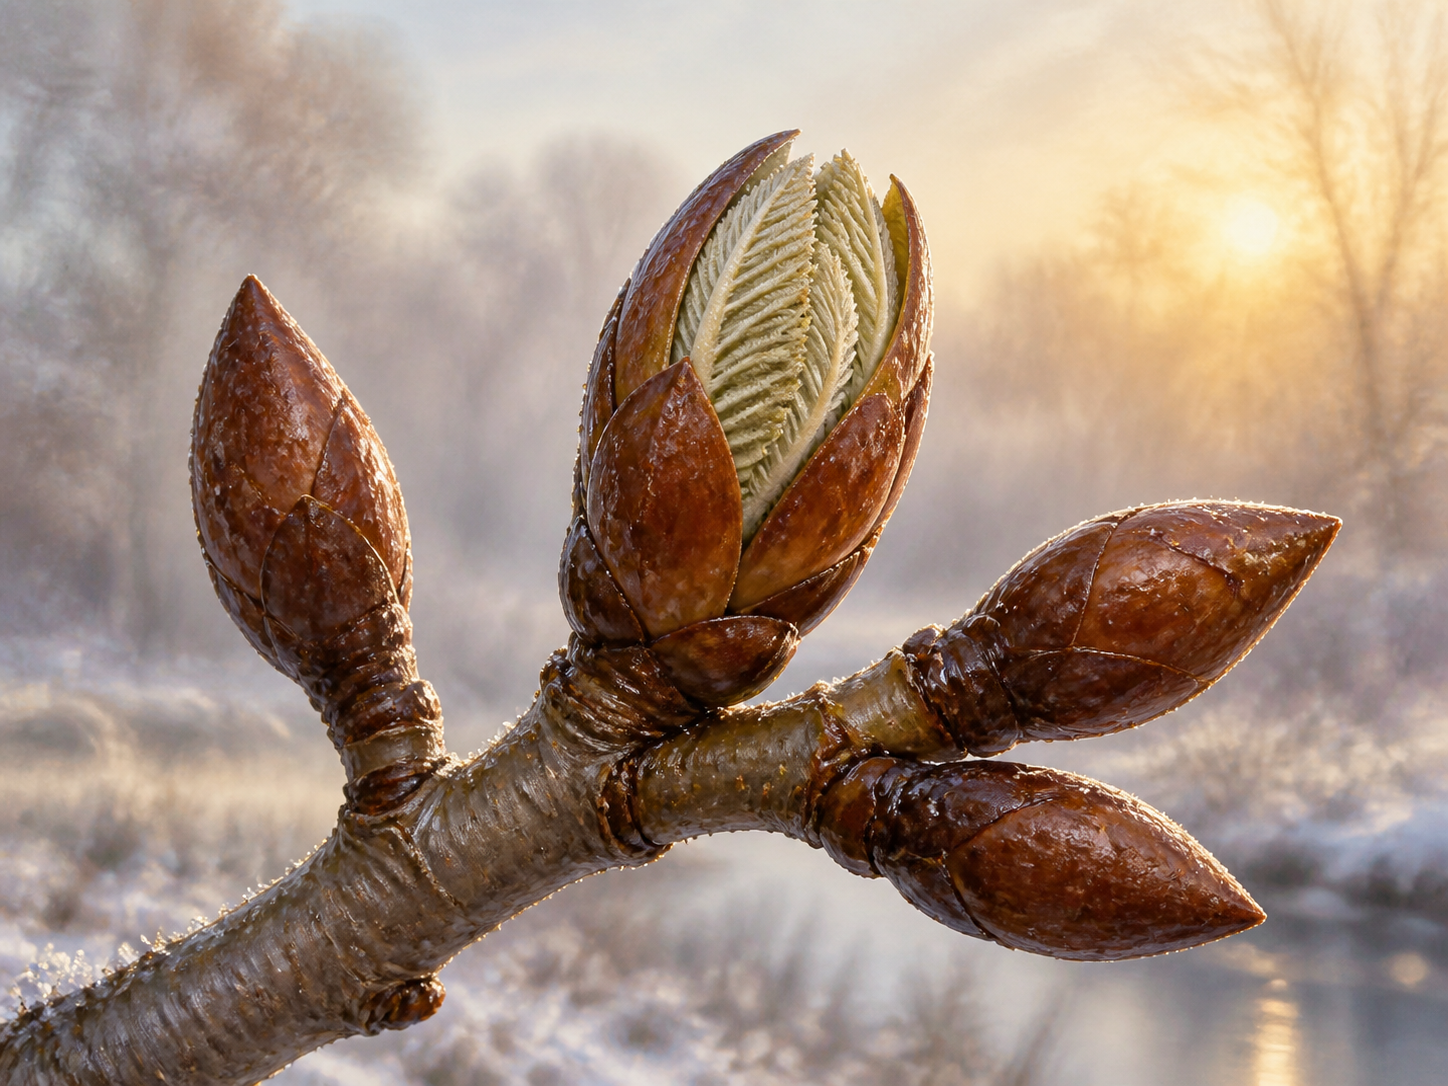
\includegraphics[width=0.56\linewidth]{images/book1/ai/g6-seasons-buds.png}

{\small Le rangement d'hiver, ouvert~: sous les \omterm{def:g1:animals-around-us:covering}{écailles} vernies du
\omterm{def:g6:life-through-seasons:buds}{bourgeon} de marronnier, les \omterm{def:g1:plants-around-us:parts}{feuilles} du printemps suivant reposent
pliées et achevées.}
\end{omfigure}

\begin{proposition}[Les réponses d'hiver de la strate herbacée]\label{prop:g6:life-through-seasons:herbs}
Les \omterm{def:g1:plants-around-us:plant}{plantes} plus petites ont leurs propres stratégies~:
\begin{itemize}
  \item les \emph{annuelles}\index{plante annuelle} --- le
        coquelicot, le haricot --- meurent entièrement en automne
        et passent l'hiver sous forme de \emph{\omterm{prop:g3:flowers-fruits-seeds:transform}{graines}}
        (\cref{prop:g2:from-seed-to-plant:needs}~: une \omterm{def:g2:from-seed-to-plant:seed}{graine}
        traverse le froid sans danger)~;
  \item les \emph{vivaces}\index{plante vivace} --- la jonquille,
        le pissenlit --- laissent mourir leur partie aérienne et
        attendent sous terre sous forme de \omterm{ex:g4:plants-without-seeds:bulbtuber}{bulbes}, de \omterm{ex:g4:plants-without-seeds:bulbtuber}{tubercules} ou
        de souches coriaces (les réserves de
        \cref{ex:g4:plants-without-seeds:bulbtuber}, de service
        d'hiver)~;
  \item les \omterm{def:g6:life-through-seasons:trees}{persistantes} du sol --- mousse, lierre --- endurent,
        tout simplement.
\end{itemize}
\end{proposition}
\admitted

\begin{example}[Où sont passées les jonquilles~?]\label{ex:g6:life-through-seasons:daffodil}
Le carré de jonquilles fleurit en mars, jaunit en mai, et en juillet
il a disparu sans laisser de trace --- et pourtant, en mars
suivant, il revient, plus dense. Tout l'été, l'automne et l'hiver,
il a existé sous forme de \omterm{ex:g4:plants-without-seeds:bulbtuber}{bulbes} sous la pelouse~: la \omterm{def:g1:plants-around-us:plant}{plante} n'est
jamais partie~; elle s'est retirée dans sa réserve.
\end{example}

\section{Le calendrier des animaux, revisité}

\begin{proposition}[Les réponses animales, en termes de relevé]\label{prop:g6:life-through-seasons:animals}
Les trois stratégies de \cref{ch:g3:animals-through-seasons} ---
\omterm{def:g3:animals-through-seasons:migration}{migrer}, \omterm{def:g3:animals-through-seasons:hibernation}{hiberner}, rester actif --- se lisent maintenant comme des
réponses aux changements relevés~: chaque \omterm{def:g5:biodiversity:species}{espèce} suit les \omterm{def:g6:exploring-our-environment:conditions}{conditions}
et la nourriture dont elle a besoin.
\begin{itemize}
  \item l'hirondelle suit son approvisionnement là où les
        \omterm{def:g6:exploring-our-environment:conditions}{conditions} gardent les \omterm{prop:g3:sorting-living-things:groups}{insectes} en vol~;
  \item le hérisson et l'escargot scellé attendent la fin des mois
        que leur corps ne peut pas traverser en activité~;
  \item les \omterm{prop:g3:sorting-living-things:groups}{insectes} ajoutent une quatrième réponse~: la plupart
        passent l'hiver sous forme d'\emph{\omterm{def:g2:animals-grow-up:born}{œufs}, de larves ou de
        \omterm{ex:g2:animals-grow-up:butterfly}{chrysalides}} (\cref{ex:g2:animals-grow-up:butterfly})
        glissés dans le sol, l'écorce ou la litière --- l'adulte
        meurt, l'\omterm{def:g5:biodiversity:species}{espèce} hiverne sous ses formes jeunes.
\end{itemize}
\end{proposition}
\admitted

\begin{example}[Où sont en janvier les insectes de juin]\label{ex:g6:life-through-seasons:insects}
La haie de janvier ne montre aucun insecte --- et pourtant ceux de
juin sont tous présents~: les papillons en \omterm{ex:g2:animals-grow-up:butterfly}{chrysalides} sous les
pierres du chaperon, les sauterelles en \omterm{def:g2:animals-grow-up:born}{œufs} dans le sol, les
coccinelles en adultes serrés et endormis au fond de la litière, les
abeilles en grappe chaude et compacte dans la ruche. Le relevé de
juin se promène~; celui de janvier doit creuser, soulever et scruter
--- les habitants ont changé de \emph{forme}, pas d'adresse.
\end{example}

\begin{method}[Relever un site tout au long de l'année]\label{met:g6:life-through-seasons:yearsurvey}
Pour étudier la vie saisonnière d'un site~:
\begin{enumerate}
  \item relève le même site marqué
        (\cref{met:g6:exploring-our-environment:survey}) une fois
        par saison --- même carré, mêmes instruments, même temps de
        recherche~;
  \item note les \omterm{def:g6:exploring-our-environment:conditions}{conditions} \emph{et} les habitants chaque fois~;
        photographie le site depuis le même point~;
  \item cherche délibérément les formes cachées de l'hiver~:
        \omterm{def:g6:life-through-seasons:buds}{bourgeons}, \omterm{ex:g4:plants-without-seeds:bulbtuber}{bulbes}, \omterm{def:g2:animals-grow-up:born}{œufs}, \omterm{ex:g2:animals-grow-up:butterfly}{chrysalides}, escargots scellés ---
        et remets chaque abri en place~;
  \item aligne les quatre relevés~: associe chaque changement
        d'habitants à un changement de \omterm{def:g6:exploring-our-environment:conditions}{conditions}, et nomme pour
        chaque absent sa forme ou sa destination d'hiver.
\end{enumerate}
\end{method}

\begin{remark}[Rien ne disparaît purement et simplement]\label{rem:g6:life-through-seasons:vanish}
Le tableau de toute l'année enseigne une règle profonde~: aucune
\omterm{def:g5:biodiversity:species}{espèce} du relevé de juin n'a simplement cessé d'être. Chacune est
ailleurs (migrée), endormie (en hibernation), en réserve (\omterm{ex:g4:plants-without-seeds:bulbtuber}{bulbe},
\omterm{def:g2:from-seed-to-plant:seed}{graine}), ou dans un autre stade de vie (\omterm{def:g2:animals-grow-up:born}{œuf}, \omterm{ex:g2:animals-grow-up:butterfly}{chrysalide}).
«~Disparu~» n'est jamais une réponse complète en \omterm{def:g1:living-or-not:living}{biologie} --- la
question qui suit est toujours~: \emph{disparu où, sous quelle
forme~?}
\end{remark}

\section{Exercices}

\begin{exercise}[$\star$]\label{exo:g6:life-through-seasons:1}
Quelles \omterm{def:g6:exploring-our-environment:conditions}{conditions} d'un site varient avec les saisons~? Nomme-en
trois.
\end{exercise}

\begin{exercise}[$\star$]\label{exo:g6:life-through-seasons:2}
\omterm{def:g6:life-through-seasons:trees}{Caduc} ou \omterm{def:g6:life-through-seasons:trees}{persistant}~: le chêne, le pin, le hêtre, le houx, le
marronnier~? Que veut dire chacun de ces mots~?
\end{exercise}

\begin{exercise}[$\star$]\label{exo:g6:life-through-seasons:3}
Qu'y a-t-il dans un \omterm{def:g6:life-through-seasons:buds}{bourgeon} d'hiver, et quand a-t-il été bâti~?
\end{exercise}

\begin{exercise}[$\star$]\label{exo:g6:life-through-seasons:4}
Comment une \omterm{prop:g6:life-through-seasons:herbs}{plante annuelle} passe-t-elle l'hiver~? Et une vivace
comme la jonquille~?
\end{exercise}

\begin{exercise}[$\star$]\label{exo:g6:life-through-seasons:5}
Explique le rameau de février de
\cref{ex:g6:life-through-seasons:bud}~: pourquoi peut-il débourrer
des semaines en avance à l'intérieur~?
\end{exercise}

\begin{exercise}[$\star$]\label{exo:g6:life-through-seasons:6}
Donne les quatre réponses d'hiver des \omterm{def:g1:animals-around-us:animal}{animaux}, chacune avec une
\omterm{def:g5:biodiversity:species}{espèce}.
\end{exercise}

\begin{exercise}[$\star\star$]\label{exo:g6:life-through-seasons:7}
Pour chaque habitant de la haie en juin, nomme sa forme et son
adresse en janvier~: papillon, sauterelle, coccinelle, escargot,
hirondelle.
\end{exercise}

\begin{exercise}[$\star\star$]\label{exo:g6:life-through-seasons:8}
Pourquoi les quatre relevés saisonniers doivent-ils employer le même
site, les mêmes instruments et le même temps de recherche~? Quelle
règle de \cref{ch:g6:exploring-our-environment} est à l'œuvre~?
\end{exercise}

\begin{exercise}[$\star\star$]\label{exo:g6:life-through-seasons:9}
Le relevé de la haie en janvier liste bien moins d'\omterm{def:g6:exploring-our-environment:components}{êtres vivants} que
celui de juin. Donne deux raisons pour lesquelles cet écart
exagère la perte réelle, en te servant de
\cref{ex:g6:life-through-seasons:insects}.
\end{exercise}

\begin{exercise}[$\star\star$]\label{exo:g6:life-through-seasons:10}
Un jardinier retourne en août le terrain «~mort~» des jonquilles et
y trouve des \omterm{ex:g4:plants-without-seeds:bulbtuber}{bulbes} fermes. Traduis cette découverte avec
\cref{prop:g6:life-through-seasons:herbs}~: dans quel état est la
\omterm{def:g1:plants-around-us:plant}{plante}, et que feront les \omterm{ex:g4:plants-without-seeds:bulbtuber}{bulbes} en mars~?
\end{exercise}

\begin{exercise}[$\star\star$]\label{exo:g6:life-through-seasons:11}
Applique \cref{rem:g6:life-through-seasons:vanish}~: les grenouilles
d'une mare sont introuvables en janvier. Donne les deux questions à
poser, et la réponse que grenouilles et crapauds y apportent.
\end{exercise}

\begin{exercise}[$\star\star\star$]\label{exo:g6:life-through-seasons:12}
Les \omterm{def:g1:plants-around-us:parts}{feuilles} \omterm{def:g6:life-through-seasons:trees}{persistantes} sont coriaces, cireuses ou en forme
d'aiguilles~; les \omterm{def:g1:plants-around-us:parts}{feuilles} \omterm{def:g6:life-through-seasons:trees}{caduques} sont larges et minces. Propose
le problème d'hiver auquel répond la construction de la \omterm{def:g1:plants-around-us:parts}{feuille}
persistante (pense aux ennuis d'eau du cloporte, à l'envers), et
dis pourquoi l'arbre à \omterm{def:g1:plants-around-us:parts}{feuilles} \omterm{def:g6:life-through-seasons:trees}{caduques} préfère laisser tomber ses
\omterm{def:g1:plants-around-us:parts}{feuilles} minces.
\end{exercise}

\section{Problème~: les douze photographies}

\begin{problem}[{Problème du week-end --- une année du marronnier,
lue image par image}]\label{pb:g6:life-through-seasons:1}
Lena photographie le marronnier près du portail le premier de chaque
mois pendant un an, et épingle les douze tirages à la suite. Sous
chaque tirage, elle note la durée du jour et la \omterm{def:g6:exploring-our-environment:conditions}{température} du
matin.

\medskip\noindent\textbf{Partie I --- Lire la série.}
\begin{enumerate}
  \item Janvier et décembre montrent des \omterm{def:g1:plants-around-us:tree}{branches} nues. Qu'y a-t-il
        sur les rameaux qui prouve, dans les deux images, que
        l'arbre est vivant et prêt pour le printemps~?
  \item Entre quelles deux images les \omterm{def:g6:life-through-seasons:buds}{bourgeons} éclatent-ils~? Les
        notes de Lena y indiquent~: des jours de $11$ à $13$
        heures, des matins de $8$ à \qty{12}{\degreeCelsius}. À
        quelles \omterm{def:g6:exploring-our-environment:conditions}{conditions} changeantes l'arbre répond-il~?
  \item L'image de mai montre des «~chandelles~» dressées de \omterm{def:g3:flowers-fruits-seeds:parts}{fleurs}
        blanches. À l'aide de \cref{ch:g3:flowers-fruits-seeds} (ou
        de \cref{ch:g5:flower-to-fruit}), que doit-il se passer
        entre les images de mai et de septembre pour que les
        marrons d'octobre existent --- et qu'est-ce qu'un marron,
        exactement~?
  \item L'image d'octobre montre des \omterm{def:g1:plants-around-us:parts}{feuilles} dorées~; celle de
        novembre, des \omterm{def:g1:plants-around-us:tree}{branches} nues et un tapis brun en dessous.
        Nomme le type de l'arbre d'après
        \cref{def:g6:life-through-seasons:trees}, et dis où est
        rangé son printemps suivant pendant les images qui suivent.
\end{enumerate}

\medskip\noindent\textbf{Partie II --- Les voisins de l'arbre.}
\begin{enumerate}[resume]
  \item Sous l'arbre, l'image de mars saisit un carré de jonquilles
        absent de celle de juillet. Où est ce carré en juillet, et
        sous quelle forme~?
  \item Des coquelicots bordent le chemin en juin~; sur l'image de
        janvier, leur emplacement est de la terre nue. Sous quelle
        forme le coquelicot est-il présent en janvier, et par
        quelle stratégie de
        \cref{prop:g6:life-through-seasons:herbs}~?
  \item L'image de juin saisit une hirondelle au-dessus de l'arbre
        et des abeilles sur les \omterm{def:g3:flowers-fruits-seeds:parts}{fleurs} en dessous~; ni l'une ni les
        autres n'apparaissent de novembre à février. Pour chacune,
        dis où elle est alors, et sous quelle forme.
  \item Une pie apparaît sur chacune des images. De quelle
        stratégie animale s'agit-il, et que la pie doit-elle gérer
        tout l'hiver, que l'hirondelle évite en partant~?
\end{enumerate}

\medskip\noindent\textbf{Partie III --- La règle de la série.}
\begin{enumerate}[resume]
  \item Lena résume~: «~l'année de l'arbre suit l'année des
        \omterm{def:g6:exploring-our-environment:conditions}{conditions}~». Appuie-la avec deux associations entre un
        changement de l'arbre d'une image à l'autre et un
        changement dans ses notes de durée du jour et de
        \omterm{def:g6:exploring-our-environment:conditions}{température}.
  \item Son petit frère dit que le carré de jonquilles de juillet
        est «~mort~». Corrige-le avec
        \cref{rem:g6:life-through-seasons:vanish} --- et énonce la
        question de suivi que son mot «~disparu~» mérite toujours.
  \item Prédis l'image 13 --- la photographie de janvier prochain
        --- en détail~: \omterm{def:g1:plants-around-us:tree}{branches}, rameaux, sol en dessous. Quelles
        parties de ta prédiction sont assez sûres pour que l'on
        parie dessus, et pourquoi~?
  \item Un rameau de marronnier, coupé en février et mis dans de
        l'eau tiède à l'intérieur, débourre en trois semaines. Que
        montre cela sur \emph{quelle} condition les \omterm{def:g6:life-through-seasons:buds}{bourgeons}
        attendaient --- et conçois l'expérience honnête à deux rameaux
        (\cref{met:g4:what-plants-need:fairtest}) qui le
        démontrerait.
\end{enumerate}
\end{problem}
